\scanpage{61}
\mspage{11}
plus des $\deleted{\widetilde\Pi_\omega}\Pi_\omega$ et $\deleted{\widetilde\Pi_i},\Pi_i$, des régions
\[
\widetilde\Sigma_r=\widetilde\Sigma_{\deleted{\unsure{r}}i\deleted{\unsure{\omega}}}^{\omega,\varepsilon}
\]
associés aux repères $r=(i,\omega,\deleted{\unsure{\bar\omega|\varpi}}\unsure{\Rightarrow|\Sigma}\varepsilon)$ de $(J,\uline{\varepsilon})$ (ou ce qui revient au $=$, de $(J,\uline{\bar\omega})$), qu'on peut identifier, géométriquement, aux \inserted{douze} triangles-drapeaux, \inserted{$\unsure{D}_r=P_\varepsilon Q_iR_{\omega i}$} \unsure{correspondants|correspondant} à la subdivision barycentrique standard de la carte dans $\Sigma$ définie par l'équateur $\Sigma_{\mathbb R}$ et par les trois points $R_i$ sur celui-ci.
\figure{
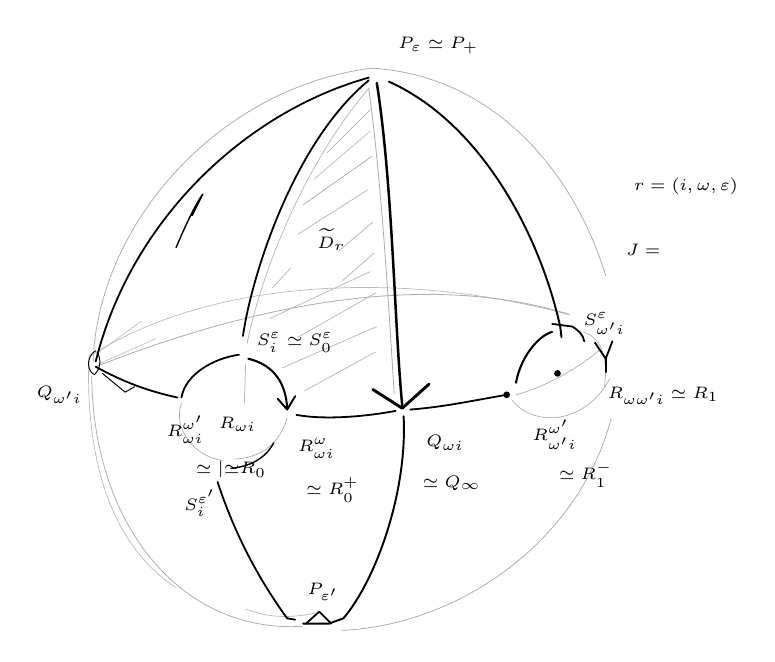
\begin{tikzpicture}[x=.017cm,y=-.017cm,line cap=round,line join=round,font=\fontsize{6}{6.5}\selectfont]
\draw[gray!65,line width=.28pt] (122,874) .. controls (126,770) and (217,669) .. (330,655) .. controls (420,660) and (481,731) .. (505,810);
\draw[gray!65,line width=.28pt] (509,917) .. controls (485,1008) and (396,1071) .. (308,1075);
\draw[gray!65,line width=.28pt] (278,1072) .. controls (188,1077) and (122,997) .. (121,885);
\draw[gray!55,line width=.25pt] (119,869) .. controls (116,935) and (130,1008) .. (184,1043);
\draw[gray!55,line width=.25pt] (236,1059) .. controls (256,1067) and (274,1065) .. (288,1062);
\draw[gray!55,line width=.25pt] (123,868) .. controls (218,809) and (363,808) .. (477,839);
\draw[gray!65,line width=.3pt] (124,878) .. controls (225,838) and (362,803) .. (478,839);
\draw[gray!50,line width=.25pt] (125,868) -- (158,844);
\draw[gray!50,line width=.25pt] (126,876) -- (169,857);
\draw[gray!55,line width=.28pt] (328,670) .. controls (284,721) and (249,801) .. (237,861);
\draw[gray!65,line width=.3pt] (328,670) .. controls (338,744) and (343,837) .. (347,898);
\draw[gray!60,line width=.28pt] (297,718) -- (329,686);
\draw[gray!50,line width=.28pt] (287,738) -- (329,702);
\draw[gray!65,line width=.28pt] (279,757) -- (330,721);
\draw[gray!55,line width=.28pt] (275,779) -- (327,746);
\draw[gray!55,line width=.28pt] (305,792) -- (331,770);
\draw[gray!55,line width=.28pt] (256,819) -- (270,804);
\draw[gray!55,line width=.28pt] (308,814) -- (332,793);
\draw[gray!55,line width=.28pt] (254,842) -- (329,807);
\draw[gray!55,line width=.28pt] (275,856) -- (333,823);
\draw[gray!55,line width=.28pt] (263,879) -- (334,848);
\draw[gray!55,line width=.28pt] (280,896) -- (333,867);
\draw[line width=.65pt] (124,874) .. controls (150,769) and (235,688) .. (328,662);
\draw[line width=.5pt] (184,789) .. controls (192,770) and (200,754) .. (204,749) -- (196,765);
\draw[line width=.7pt] (343,665) .. controls (410,695) and (455,776) .. (471,848) -- (472,856);
\draw[line width=.65pt] (328,664) .. controls (271,711) and (240,812) .. (234,855);
\draw[line width=.9pt] (334,666) .. controls (346,743) and (347,845) .. (353,907);
\draw[line width=1.05pt] (331,895) -- (353,909) -- (373,891);
\draw[line width=.7pt] (354,915) .. controls (357,972) and (333,1038) .. (309,1066) -- (298,1070) -- (279,1070);
\draw[line width=.65pt] (215,964) .. controls (230,1010) and (251,1044) .. (267,1066) -- (273,1067);
\draw[line width=.65pt] (281,1070) -- (291,1061) -- (300,1070);
\draw[line width=.65pt] (124,878) .. controls (144,889) and (162,896) .. (185,901);
\draw[line width=.35pt] (129,883) -- (146,897) -- (153,893);
\draw[line width=.35pt] (124,866) .. controls (117,870) and (117,881) .. (123,884) .. controls (128,879) and (128,872) .. (125,867);
\draw[line width=.65pt] (188,901) .. controls (191,884) and (211,872) .. (231,869);
\draw[line width=.75pt] (238,872) .. controls (258,877) and (266,891) .. (267,909);
\draw[line width=.7pt] (260,902) -- (267,910) -- (273,900);
\draw[gray!65,line width=.25pt] (188,905) .. controls (181,925) and (199,946) .. (219,948);
\draw[gray!65,line width=.25pt] (228,947) .. controls (249,946) and (262,934) .. (267,916);
\draw[line width=.5pt] (225,954) .. controls (243,952) and (252,944) .. (257,935);
\draw[gray!60,line width=.25pt] (236,876) -- (235,906);
\draw[line width=.65pt] (274,914) .. controls (296,918) and (327,915) .. (348,911);
\draw[line width=.65pt] (359,910) .. controls (385,908) and (407,903) .. (431,899);
\draw[gray!65,line width=.25pt] (435,903) .. controls (451,923) and (489,922) .. (508,887);
\draw[gray!65,line width=.25pt] (488,852) .. controls (502,856) and (507,872) .. (504,893);
\draw[gray!65,line width=.25pt] (438,899) .. controls (460,893) and (485,879) .. (501,865);
\draw[line width=.75pt] (438,890) .. controls (441,872) and (454,855) .. (465,852);
\draw[line width=.65pt] (465,846) -- (480,848) .. controls (485,851) and (488,854) .. (489,859);
\draw[line width=.65pt] (497,860) -- (505,872) -- (510,859);
\draw[line width=.65pt] (505,872) -- (505,882);
\fill (431,899) circle[radius=.425mm];
\fill (469,883) circle[radius=.425mm];
\node at (380,638) {$P_\varepsilon\simeq P_+$};
\node at (300,783) {$\widetilde{\unsure{D}}_r$};
\node[anchor=east] at (121,899) {$Q_{\omega'i}$};
\node[anchor=west] at (237,860) {$S_i^\varepsilon\simeq S_0^\varepsilon$};
\node at (191,925) {$R_{\omega i}^{\omega'}$};
\node at (289,939) {$R_{\unsure{\omega i}}^\omega$};
\node at (301,970) {$\simeq R_0^+$};
\node at (230,921) {$\unsure{R}_{\deleted{\unsure{\omega}}i}$};
\node at (225,955) {$\unsure{\simeq|\deleted{\simeq}}\deleted{\unsure{R_0}}$};
\node at (202,980) {$S_i^{\varepsilon'}$};
\node at (385,935) {$Q_{\deleted{\unsure{\omega}}i}$};
\node at (390,965) {$\simeq Q_\infty$};
\node at (504,846) {$S_{\omega'i}^\varepsilon$};
\node at (548,900) {$R_{\deleted{\unsure{\omega}}\unsure{\omega'}i}\simeq R_1$};
\node at (467,929) {$R_{\unsure{\omega'i}}^{\omega'}$};
\node at (490,959) {$\simeq R_1^-$};
\node at (294,1046) {$P_{\varepsilon'}$};
\node at (565,743) {$r=(i,\omega,\varepsilon)$};
\node at (533,791) {$J=$};
\end{tikzpicture}}
Le ``tronc'' \inserted{sur $\widetilde\Sigma$} au sens évident d'un tel triangle est un quadrilatère $\widetilde D_r$
\[
P_\varepsilon Q_{\omega'i}R_i^\omega S_i^\varepsilon\unsure{.}\simeq P_+Q_\infty R_0^+S_0^+.
\]
On aura à travail-\linebreak ler, au ``voisinage'' immédiat'' de \unsure{ces|ce} \deleted{\unsure{repères|repère}} \inserted{drapeaux} \deleted{\unsure{triangles des}} $\widetilde\Sigma_r$, avec les symétriques de $\Sigma_r$ p.r. à ses trois côtés, et se trouve sur $\widetilde\Sigma_{\unsure{\deleted{r}|r}}$, \deleted{\unsure{pour ce qui}} \inserted{ce qui conduit} à regarder la réunion de $\Sigma_r$ avec ses trois frères
\[
\tau(\Sigma_r),\widetilde\sigma_i(\Sigma_r),\widetilde\sigma_{\omega i}(\Sigma_r)
\]
(qui \inserted{resp.} correspondent, sur la sphère standard avec le repère correspondant au triangle $P_+Q_\infty R_0$, à $\tau,\widetilde\sigma_\infty,\widetilde\sigma_0$) et sur $\widetilde\Sigma$ à prendre
\[
(41)\qquad\widetilde\Sigma_r=\widetilde\Sigma_i^{\omega,\varepsilon}=\widetilde D_r\cup\tau(\widetilde D_r)\cup\widetilde\sigma_i(\widetilde D_r)\cup\widetilde\sigma_{\omega i}(\Sigma_+)
\]
limités par le contour
\[
P_\varepsilon Q_{\omega'i}R_{\omega i}^{\omega'}S_i^\varepsilon R_{\omega i}^\omega S_i^{\varepsilon'}P_{\varepsilon'}Q_iR_{\unsure{\omega'i|\omega^2i}}^{\omega'}S_{\unsure{\omega'i|\omega^2i}}^\varepsilon P_\varepsilon
\]
\margin{60}
